% Options for packages loaded elsewhere
% Options for packages loaded elsewhere
\PassOptionsToPackage{unicode}{hyperref}
\PassOptionsToPackage{hyphens}{url}
\PassOptionsToPackage{dvipsnames,svgnames,x11names}{xcolor}
%
\documentclass[
  letterpaper,
  DIV=11,
  numbers=noendperiod]{scrartcl}
\usepackage{xcolor}
\usepackage{amsmath,amssymb}
\setcounter{secnumdepth}{-\maxdimen} % remove section numbering
\usepackage{iftex}
\ifPDFTeX
  \usepackage[T1]{fontenc}
  \usepackage[utf8]{inputenc}
  \usepackage{textcomp} % provide euro and other symbols
\else % if luatex or xetex
  \usepackage{unicode-math} % this also loads fontspec
  \defaultfontfeatures{Scale=MatchLowercase}
  \defaultfontfeatures[\rmfamily]{Ligatures=TeX,Scale=1}
\fi
\usepackage{lmodern}
\ifPDFTeX\else
  % xetex/luatex font selection
\fi
% Use upquote if available, for straight quotes in verbatim environments
\IfFileExists{upquote.sty}{\usepackage{upquote}}{}
\IfFileExists{microtype.sty}{% use microtype if available
  \usepackage[]{microtype}
  \UseMicrotypeSet[protrusion]{basicmath} % disable protrusion for tt fonts
}{}
\makeatletter
\@ifundefined{KOMAClassName}{% if non-KOMA class
  \IfFileExists{parskip.sty}{%
    \usepackage{parskip}
  }{% else
    \setlength{\parindent}{0pt}
    \setlength{\parskip}{6pt plus 2pt minus 1pt}}
}{% if KOMA class
  \KOMAoptions{parskip=half}}
\makeatother
% Make \paragraph and \subparagraph free-standing
\makeatletter
\ifx\paragraph\undefined\else
  \let\oldparagraph\paragraph
  \renewcommand{\paragraph}{
    \@ifstar
      \xxxParagraphStar
      \xxxParagraphNoStar
  }
  \newcommand{\xxxParagraphStar}[1]{\oldparagraph*{#1}\mbox{}}
  \newcommand{\xxxParagraphNoStar}[1]{\oldparagraph{#1}\mbox{}}
\fi
\ifx\subparagraph\undefined\else
  \let\oldsubparagraph\subparagraph
  \renewcommand{\subparagraph}{
    \@ifstar
      \xxxSubParagraphStar
      \xxxSubParagraphNoStar
  }
  \newcommand{\xxxSubParagraphStar}[1]{\oldsubparagraph*{#1}\mbox{}}
  \newcommand{\xxxSubParagraphNoStar}[1]{\oldsubparagraph{#1}\mbox{}}
\fi
\makeatother

\usepackage{color}
\usepackage{fancyvrb}
\newcommand{\VerbBar}{|}
\newcommand{\VERB}{\Verb[commandchars=\\\{\}]}
\DefineVerbatimEnvironment{Highlighting}{Verbatim}{commandchars=\\\{\}}
% Add ',fontsize=\small' for more characters per line
\usepackage{framed}
\definecolor{shadecolor}{RGB}{241,243,245}
\newenvironment{Shaded}{\begin{snugshade}}{\end{snugshade}}
\newcommand{\AlertTok}[1]{\textcolor[rgb]{0.68,0.00,0.00}{#1}}
\newcommand{\AnnotationTok}[1]{\textcolor[rgb]{0.37,0.37,0.37}{#1}}
\newcommand{\AttributeTok}[1]{\textcolor[rgb]{0.40,0.45,0.13}{#1}}
\newcommand{\BaseNTok}[1]{\textcolor[rgb]{0.68,0.00,0.00}{#1}}
\newcommand{\BuiltInTok}[1]{\textcolor[rgb]{0.00,0.23,0.31}{#1}}
\newcommand{\CharTok}[1]{\textcolor[rgb]{0.13,0.47,0.30}{#1}}
\newcommand{\CommentTok}[1]{\textcolor[rgb]{0.37,0.37,0.37}{#1}}
\newcommand{\CommentVarTok}[1]{\textcolor[rgb]{0.37,0.37,0.37}{\textit{#1}}}
\newcommand{\ConstantTok}[1]{\textcolor[rgb]{0.56,0.35,0.01}{#1}}
\newcommand{\ControlFlowTok}[1]{\textcolor[rgb]{0.00,0.23,0.31}{\textbf{#1}}}
\newcommand{\DataTypeTok}[1]{\textcolor[rgb]{0.68,0.00,0.00}{#1}}
\newcommand{\DecValTok}[1]{\textcolor[rgb]{0.68,0.00,0.00}{#1}}
\newcommand{\DocumentationTok}[1]{\textcolor[rgb]{0.37,0.37,0.37}{\textit{#1}}}
\newcommand{\ErrorTok}[1]{\textcolor[rgb]{0.68,0.00,0.00}{#1}}
\newcommand{\ExtensionTok}[1]{\textcolor[rgb]{0.00,0.23,0.31}{#1}}
\newcommand{\FloatTok}[1]{\textcolor[rgb]{0.68,0.00,0.00}{#1}}
\newcommand{\FunctionTok}[1]{\textcolor[rgb]{0.28,0.35,0.67}{#1}}
\newcommand{\ImportTok}[1]{\textcolor[rgb]{0.00,0.46,0.62}{#1}}
\newcommand{\InformationTok}[1]{\textcolor[rgb]{0.37,0.37,0.37}{#1}}
\newcommand{\KeywordTok}[1]{\textcolor[rgb]{0.00,0.23,0.31}{\textbf{#1}}}
\newcommand{\NormalTok}[1]{\textcolor[rgb]{0.00,0.23,0.31}{#1}}
\newcommand{\OperatorTok}[1]{\textcolor[rgb]{0.37,0.37,0.37}{#1}}
\newcommand{\OtherTok}[1]{\textcolor[rgb]{0.00,0.23,0.31}{#1}}
\newcommand{\PreprocessorTok}[1]{\textcolor[rgb]{0.68,0.00,0.00}{#1}}
\newcommand{\RegionMarkerTok}[1]{\textcolor[rgb]{0.00,0.23,0.31}{#1}}
\newcommand{\SpecialCharTok}[1]{\textcolor[rgb]{0.37,0.37,0.37}{#1}}
\newcommand{\SpecialStringTok}[1]{\textcolor[rgb]{0.13,0.47,0.30}{#1}}
\newcommand{\StringTok}[1]{\textcolor[rgb]{0.13,0.47,0.30}{#1}}
\newcommand{\VariableTok}[1]{\textcolor[rgb]{0.07,0.07,0.07}{#1}}
\newcommand{\VerbatimStringTok}[1]{\textcolor[rgb]{0.13,0.47,0.30}{#1}}
\newcommand{\WarningTok}[1]{\textcolor[rgb]{0.37,0.37,0.37}{\textit{#1}}}

\usepackage{longtable,booktabs,array}
\usepackage{calc} % for calculating minipage widths
% Correct order of tables after \paragraph or \subparagraph
\usepackage{etoolbox}
\makeatletter
\patchcmd\longtable{\par}{\if@noskipsec\mbox{}\fi\par}{}{}
\makeatother
% Allow footnotes in longtable head/foot
\IfFileExists{footnotehyper.sty}{\usepackage{footnotehyper}}{\usepackage{footnote}}
\makesavenoteenv{longtable}
\usepackage{graphicx}
\makeatletter
\newsavebox\pandoc@box
\newcommand*\pandocbounded[1]{% scales image to fit in text height/width
  \sbox\pandoc@box{#1}%
  \Gscale@div\@tempa{\textheight}{\dimexpr\ht\pandoc@box+\dp\pandoc@box\relax}%
  \Gscale@div\@tempb{\linewidth}{\wd\pandoc@box}%
  \ifdim\@tempb\p@<\@tempa\p@\let\@tempa\@tempb\fi% select the smaller of both
  \ifdim\@tempa\p@<\p@\scalebox{\@tempa}{\usebox\pandoc@box}%
  \else\usebox{\pandoc@box}%
  \fi%
}
% Set default figure placement to htbp
\def\fps@figure{htbp}
\makeatother





\setlength{\emergencystretch}{3em} % prevent overfull lines

\providecommand{\tightlist}{%
  \setlength{\itemsep}{0pt}\setlength{\parskip}{0pt}}



 


\KOMAoption{captions}{tableheading}
\makeatletter
\@ifpackageloaded{caption}{}{\usepackage{caption}}
\AtBeginDocument{%
\ifdefined\contentsname
  \renewcommand*\contentsname{Table of contents}
\else
  \newcommand\contentsname{Table of contents}
\fi
\ifdefined\listfigurename
  \renewcommand*\listfigurename{List of Figures}
\else
  \newcommand\listfigurename{List of Figures}
\fi
\ifdefined\listtablename
  \renewcommand*\listtablename{List of Tables}
\else
  \newcommand\listtablename{List of Tables}
\fi
\ifdefined\figurename
  \renewcommand*\figurename{Figure}
\else
  \newcommand\figurename{Figure}
\fi
\ifdefined\tablename
  \renewcommand*\tablename{Table}
\else
  \newcommand\tablename{Table}
\fi
}
\@ifpackageloaded{float}{}{\usepackage{float}}
\floatstyle{ruled}
\@ifundefined{c@chapter}{\newfloat{codelisting}{h}{lop}}{\newfloat{codelisting}{h}{lop}[chapter]}
\floatname{codelisting}{Listing}
\newcommand*\listoflistings{\listof{codelisting}{List of Listings}}
\makeatother
\makeatletter
\makeatother
\makeatletter
\@ifpackageloaded{caption}{}{\usepackage{caption}}
\@ifpackageloaded{subcaption}{}{\usepackage{subcaption}}
\makeatother
\usepackage{bookmark}
\IfFileExists{xurl.sty}{\usepackage{xurl}}{} % add URL line breaks if available
\urlstyle{same}
\hypersetup{
  pdftitle={Simulation Challenge},
  colorlinks=true,
  linkcolor={blue},
  filecolor={Maroon},
  citecolor={Blue},
  urlcolor={Blue},
  pdfcreator={LaTeX via pandoc}}


\title{Simulation Challenge}
\usepackage{etoolbox}
\makeatletter
\providecommand{\subtitle}[1]{% add subtitle to \maketitle
  \apptocmd{\@title}{\par {\large #1 \par}}{}{}
}
\makeatother
\subtitle{Monte Carlo Analysis}
\author{}
\date{}
\begin{document}
\maketitle


\section{Simulation Challenge}\label{simulation-challenge}

\subsection{The Investment Game}\label{the-investment-game}

\subsubsection{Original Game Strategy}\label{original-game-strategy}

You are given \$1,000 to play this game: Flip a coin each year until age
55. If heads, increase your balance by 50\%. If tails, reduce your
balance by 40\%.

\subsubsection{Modified Game Strategy}\label{modified-game-strategy}

Same as above, but you must bet exactly 50\% of your current balance on
each flip.

\subsection{Questions to Answer}\label{questions-to-answer}

\subsubsection{75\% Grade}\label{grade}

\begin{enumerate}
\def\labelenumi{\arabic{enumi}.}
\tightlist
\item
  \textbf{Expected Value Analysis:} What is the expected value after 1
  coin flip for the original game?
\end{enumerate}

\begin{Shaded}
\begin{Highlighting}[]
\CommentTok{\# Parameters for the original game}
\NormalTok{initial\_balance }\OtherTok{\textless{}{-}} \DecValTok{1000}
\NormalTok{heads\_multiplier }\OtherTok{\textless{}{-}} \FloatTok{1.5}  \CommentTok{\# +50\% gain}
\NormalTok{tails\_multiplier }\OtherTok{\textless{}{-}} \FloatTok{0.6}  \CommentTok{\# {-}40\% loss}
\NormalTok{probability\_heads }\OtherTok{\textless{}{-}} \FloatTok{0.5}

\CommentTok{\# Calculate possible outcomes after 1 coin flip}
\NormalTok{heads\_outcome }\OtherTok{\textless{}{-}}\NormalTok{ initial\_balance }\SpecialCharTok{*}\NormalTok{ heads\_multiplier}
\NormalTok{tails\_outcome }\OtherTok{\textless{}{-}}\NormalTok{ initial\_balance }\SpecialCharTok{*}\NormalTok{ tails\_multiplier}

\CommentTok{\# Calculate expected value}
\NormalTok{expected\_value }\OtherTok{\textless{}{-}}\NormalTok{ probability\_heads }\SpecialCharTok{*}\NormalTok{ heads\_outcome }\SpecialCharTok{+}\NormalTok{ (}\DecValTok{1} \SpecialCharTok{{-}}\NormalTok{ probability\_heads) }\SpecialCharTok{*}\NormalTok{ tails\_outcome}

\CommentTok{\# Display results}
\FunctionTok{cat}\NormalTok{(}\StringTok{"Expected Value Analysis (1 coin flip):}\SpecialCharTok{\textbackslash{}n}\StringTok{"}\NormalTok{)}
\end{Highlighting}
\end{Shaded}

\begin{verbatim}
Expected Value Analysis (1 coin flip):
\end{verbatim}

\begin{Shaded}
\begin{Highlighting}[]
\FunctionTok{cat}\NormalTok{(}\StringTok{"=====================================}\SpecialCharTok{\textbackslash{}n}\StringTok{"}\NormalTok{)}
\end{Highlighting}
\end{Shaded}

\begin{verbatim}
=====================================
\end{verbatim}

\begin{Shaded}
\begin{Highlighting}[]
\FunctionTok{cat}\NormalTok{(}\StringTok{"Initial balance: $"}\NormalTok{, initial\_balance, }\StringTok{"}\SpecialCharTok{\textbackslash{}n}\StringTok{"}\NormalTok{, }\AttributeTok{sep =} \StringTok{""}\NormalTok{)}
\end{Highlighting}
\end{Shaded}

\begin{verbatim}
Initial balance: $1000
\end{verbatim}

\begin{Shaded}
\begin{Highlighting}[]
\FunctionTok{cat}\NormalTok{(}\StringTok{"Heads outcome (50\% gain): $"}\NormalTok{, heads\_outcome, }\StringTok{"}\SpecialCharTok{\textbackslash{}n}\StringTok{"}\NormalTok{, }\AttributeTok{sep =} \StringTok{""}\NormalTok{)}
\end{Highlighting}
\end{Shaded}

\begin{verbatim}
Heads outcome (50% gain): $1500
\end{verbatim}

\begin{Shaded}
\begin{Highlighting}[]
\FunctionTok{cat}\NormalTok{(}\StringTok{"Tails outcome (40\% loss): $"}\NormalTok{, tails\_outcome, }\StringTok{"}\SpecialCharTok{\textbackslash{}n}\StringTok{"}\NormalTok{, }\AttributeTok{sep =} \StringTok{""}\NormalTok{)}
\end{Highlighting}
\end{Shaded}

\begin{verbatim}
Tails outcome (40% loss): $600
\end{verbatim}

\begin{Shaded}
\begin{Highlighting}[]
\FunctionTok{cat}\NormalTok{(}\StringTok{"Probability of heads: "}\NormalTok{, probability\_heads, }\StringTok{"}\SpecialCharTok{\textbackslash{}n}\StringTok{"}\NormalTok{, }\AttributeTok{sep =} \StringTok{""}\NormalTok{)}
\end{Highlighting}
\end{Shaded}

\begin{verbatim}
Probability of heads: 0.5
\end{verbatim}

\begin{Shaded}
\begin{Highlighting}[]
\FunctionTok{cat}\NormalTok{(}\StringTok{"Probability of tails: "}\NormalTok{, }\DecValTok{1} \SpecialCharTok{{-}}\NormalTok{ probability\_heads, }\StringTok{"}\SpecialCharTok{\textbackslash{}n}\StringTok{"}\NormalTok{, }\AttributeTok{sep =} \StringTok{""}\NormalTok{)}
\end{Highlighting}
\end{Shaded}

\begin{verbatim}
Probability of tails: 0.5
\end{verbatim}

\begin{Shaded}
\begin{Highlighting}[]
\FunctionTok{cat}\NormalTok{(}\StringTok{"}\SpecialCharTok{\textbackslash{}n}\StringTok{Expected Value = P(Heads) × Heads\_Outcome + P(Tails) × Tails\_Outcome}\SpecialCharTok{\textbackslash{}n}\StringTok{"}\NormalTok{)}
\end{Highlighting}
\end{Shaded}

\begin{verbatim}

Expected Value = P(Heads) × Heads_Outcome + P(Tails) × Tails_Outcome
\end{verbatim}

\begin{Shaded}
\begin{Highlighting}[]
\FunctionTok{cat}\NormalTok{(}\StringTok{"Expected Value = "}\NormalTok{, probability\_heads, }\StringTok{" × $"}\NormalTok{, heads\_outcome, }\StringTok{" + "}\NormalTok{, }\DecValTok{1} \SpecialCharTok{{-}}\NormalTok{ probability\_heads, }\StringTok{" × $"}\NormalTok{, tails\_outcome, }\StringTok{"}\SpecialCharTok{\textbackslash{}n}\StringTok{"}\NormalTok{, }\AttributeTok{sep =} \StringTok{""}\NormalTok{)}
\end{Highlighting}
\end{Shaded}

\begin{verbatim}
Expected Value = 0.5 × $1500 + 0.5 × $600
\end{verbatim}

\begin{Shaded}
\begin{Highlighting}[]
\FunctionTok{cat}\NormalTok{(}\StringTok{"Expected Value = $"}\NormalTok{, expected\_value, }\StringTok{"}\SpecialCharTok{\textbackslash{}n}\StringTok{"}\NormalTok{, }\AttributeTok{sep =} \StringTok{""}\NormalTok{)}
\end{Highlighting}
\end{Shaded}

\begin{verbatim}
Expected Value = $1050
\end{verbatim}

\begin{Shaded}
\begin{Highlighting}[]
\FunctionTok{cat}\NormalTok{(}\StringTok{"}\SpecialCharTok{\textbackslash{}n}\StringTok{Answer: The expected value after 1 coin flip is $"}\NormalTok{, expected\_value, }\StringTok{"}\SpecialCharTok{\textbackslash{}n}\StringTok{"}\NormalTok{, }\AttributeTok{sep =} \StringTok{""}\NormalTok{)}
\end{Highlighting}
\end{Shaded}

\begin{verbatim}

Answer: The expected value after 1 coin flip is $1050
\end{verbatim}

\textbf{Discussion of Results:}

The expected value analysis reveals a counterintuitive but
mathematically sound result: despite the asymmetric nature of the game
(50\% gain vs.~40\% loss), the expected value is positive at \$1,050.
This represents a 5\% expected return per coin flip, which seems
favorable at first glance. However, this analysis only considers the
average outcome over many trials. In reality, the multiplicative nature
of the game creates significant volatility - a single bad streak of
tails could dramatically reduce your balance, while a streak of heads
could lead to substantial gains. The expected value calculation assumes
we can play this game many times, but in practice, you only get one
sequence of coin flips until age 55. This highlights the important
distinction between expected value (what happens on average) and actual
outcomes (what happens in your specific case), which is a key concept in
understanding why this seemingly profitable game might not be as
attractive as it initially appears.

\begin{enumerate}
\def\labelenumi{\arabic{enumi}.}
\setcounter{enumi}{1}
\tightlist
\item
  \textbf{Expectation vs.~Reality:} Is the expected value positive or
  negative? Do you expect your account to be worth more or less than
  \$1,000?
\end{enumerate}

\begin{Shaded}
\begin{Highlighting}[]
\CommentTok{\# Use the same parameters from Question 1}
\NormalTok{initial\_balance }\OtherTok{\textless{}{-}} \DecValTok{1000}
\NormalTok{expected\_value }\OtherTok{\textless{}{-}} \DecValTok{1050}  \CommentTok{\# From previous calculation}

\CommentTok{\# Calculate the difference from initial balance}
\NormalTok{expected\_difference }\OtherTok{\textless{}{-}}\NormalTok{ expected\_value }\SpecialCharTok{{-}}\NormalTok{ initial\_balance}
\NormalTok{expected\_return\_percent }\OtherTok{\textless{}{-}}\NormalTok{ (expected\_difference }\SpecialCharTok{/}\NormalTok{ initial\_balance) }\SpecialCharTok{*} \DecValTok{100}

\CommentTok{\# Analysis}
\FunctionTok{cat}\NormalTok{(}\StringTok{"Expectation vs. Reality Analysis:}\SpecialCharTok{\textbackslash{}n}\StringTok{"}\NormalTok{)}
\end{Highlighting}
\end{Shaded}

\begin{verbatim}
Expectation vs. Reality Analysis:
\end{verbatim}

\begin{Shaded}
\begin{Highlighting}[]
\FunctionTok{cat}\NormalTok{(}\StringTok{"===============================}\SpecialCharTok{\textbackslash{}n}\StringTok{"}\NormalTok{)}
\end{Highlighting}
\end{Shaded}

\begin{verbatim}
===============================
\end{verbatim}

\begin{Shaded}
\begin{Highlighting}[]
\FunctionTok{cat}\NormalTok{(}\StringTok{"Initial balance: $"}\NormalTok{, initial\_balance, }\StringTok{"}\SpecialCharTok{\textbackslash{}n}\StringTok{"}\NormalTok{, }\AttributeTok{sep =} \StringTok{""}\NormalTok{)}
\end{Highlighting}
\end{Shaded}

\begin{verbatim}
Initial balance: $1000
\end{verbatim}

\begin{Shaded}
\begin{Highlighting}[]
\FunctionTok{cat}\NormalTok{(}\StringTok{"Expected value after 1 flip: $"}\NormalTok{, expected\_value, }\StringTok{"}\SpecialCharTok{\textbackslash{}n}\StringTok{"}\NormalTok{, }\AttributeTok{sep =} \StringTok{""}\NormalTok{)}
\end{Highlighting}
\end{Shaded}

\begin{verbatim}
Expected value after 1 flip: $1050
\end{verbatim}

\begin{Shaded}
\begin{Highlighting}[]
\FunctionTok{cat}\NormalTok{(}\StringTok{"Expected difference: $"}\NormalTok{, expected\_difference, }\StringTok{"}\SpecialCharTok{\textbackslash{}n}\StringTok{"}\NormalTok{, }\AttributeTok{sep =} \StringTok{""}\NormalTok{)}
\end{Highlighting}
\end{Shaded}

\begin{verbatim}
Expected difference: $50
\end{verbatim}

\begin{Shaded}
\begin{Highlighting}[]
\FunctionTok{cat}\NormalTok{(}\StringTok{"Expected return: "}\NormalTok{, expected\_return\_percent, }\StringTok{"\%}\SpecialCharTok{\textbackslash{}n}\StringTok{"}\NormalTok{, }\AttributeTok{sep =} \StringTok{""}\NormalTok{)}
\end{Highlighting}
\end{Shaded}

\begin{verbatim}
Expected return: 5%
\end{verbatim}

\begin{Shaded}
\begin{Highlighting}[]
\FunctionTok{cat}\NormalTok{(}\StringTok{"}\SpecialCharTok{\textbackslash{}n}\StringTok{"}\NormalTok{)}
\end{Highlighting}
\end{Shaded}

\begin{Shaded}
\begin{Highlighting}[]
\CommentTok{\# Determine if positive or negative}
\ControlFlowTok{if}\NormalTok{ (expected\_difference }\SpecialCharTok{\textgreater{}} \DecValTok{0}\NormalTok{) \{}
  \FunctionTok{cat}\NormalTok{(}\StringTok{"✓ The expected value is POSITIVE}\SpecialCharTok{\textbackslash{}n}\StringTok{"}\NormalTok{)}
  \FunctionTok{cat}\NormalTok{(}\StringTok{"✓ You expect your account to be worth MORE than $1,000}\SpecialCharTok{\textbackslash{}n}\StringTok{"}\NormalTok{)}
  \FunctionTok{cat}\NormalTok{(}\StringTok{"✓ Expected gain: $"}\NormalTok{, expected\_difference, }\StringTok{" ("}\NormalTok{, expected\_return\_percent, }\StringTok{"\%)}\SpecialCharTok{\textbackslash{}n}\StringTok{"}\NormalTok{, }\AttributeTok{sep =} \StringTok{""}\NormalTok{)}
\NormalTok{\} }\ControlFlowTok{else} \ControlFlowTok{if}\NormalTok{ (expected\_difference }\SpecialCharTok{\textless{}} \DecValTok{0}\NormalTok{) \{}
  \FunctionTok{cat}\NormalTok{(}\StringTok{"✗ The expected value is NEGATIVE}\SpecialCharTok{\textbackslash{}n}\StringTok{"}\NormalTok{)}
  \FunctionTok{cat}\NormalTok{(}\StringTok{"✗ You expect your account to be worth LESS than $1,000}\SpecialCharTok{\textbackslash{}n}\StringTok{"}\NormalTok{)}
  \FunctionTok{cat}\NormalTok{(}\StringTok{"✗ Expected loss: $"}\NormalTok{, }\FunctionTok{abs}\NormalTok{(expected\_difference), }\StringTok{" ("}\NormalTok{, }\FunctionTok{abs}\NormalTok{(expected\_return\_percent), }\StringTok{"\%)}\SpecialCharTok{\textbackslash{}n}\StringTok{"}\NormalTok{, }\AttributeTok{sep =} \StringTok{""}\NormalTok{)}
\NormalTok{\} }\ControlFlowTok{else}\NormalTok{ \{}
  \FunctionTok{cat}\NormalTok{(}\StringTok{"= The expected value is ZERO}\SpecialCharTok{\textbackslash{}n}\StringTok{"}\NormalTok{)}
  \FunctionTok{cat}\NormalTok{(}\StringTok{"= You expect your account to be worth the SAME as $1,000}\SpecialCharTok{\textbackslash{}n}\StringTok{"}\NormalTok{)}
\NormalTok{\}}
\end{Highlighting}
\end{Shaded}

\begin{verbatim}
✓ The expected value is POSITIVE
✓ You expect your account to be worth MORE than $1,000
✓ Expected gain: $50 (5%)
\end{verbatim}

\begin{Shaded}
\begin{Highlighting}[]
\FunctionTok{cat}\NormalTok{(}\StringTok{"}\SpecialCharTok{\textbackslash{}n}\StringTok{Key Insight:}\SpecialCharTok{\textbackslash{}n}\StringTok{"}\NormalTok{)}
\end{Highlighting}
\end{Shaded}

\begin{verbatim}

Key Insight:
\end{verbatim}

\begin{Shaded}
\begin{Highlighting}[]
\FunctionTok{cat}\NormalTok{(}\StringTok{"The positive expected value suggests this game is theoretically favorable.}\SpecialCharTok{\textbackslash{}n}\StringTok{"}\NormalTok{)}
\end{Highlighting}
\end{Shaded}

\begin{verbatim}
The positive expected value suggests this game is theoretically favorable.
\end{verbatim}

\begin{Shaded}
\begin{Highlighting}[]
\FunctionTok{cat}\NormalTok{(}\StringTok{"However, this is just the average outcome {-} your actual result could be very different!}\SpecialCharTok{\textbackslash{}n}\StringTok{"}\NormalTok{)}
\end{Highlighting}
\end{Shaded}

\begin{verbatim}
However, this is just the average outcome - your actual result could be very different!
\end{verbatim}

\textbf{Discussion of Results:}

The expectation vs.~reality analysis confirms that the game appears
mathematically favorable with a positive expected value of \$1,050,
representing a 5\% expected return per coin flip. This suggests that, on
average, players should expect to gain money. However, this analysis
reveals a critical gap between theoretical expectations and practical
outcomes. The positive expected value is based on the assumption that
you can play this game many times, allowing the law of large numbers to
work in your favor. In reality, you only get one sequence of coin flips
from your current age until 55, which means you're subject to the full
volatility of the game without the benefit of averaging. This creates a
paradox: while the game is theoretically profitable, the high variance
means you could easily end up with significantly less than your initial
\$1,000 investment. The 5\% expected return per flip sounds attractive,
but it doesn't account for the risk of ruin or the psychological impact
of potentially large losses. This highlights why expected value alone is
insufficient for decision-making in high-variance scenarios - you need
to consider the entire distribution of possible outcomes, not just the
average.

\begin{enumerate}
\def\labelenumi{\arabic{enumi}.}
\setcounter{enumi}{2}
\tightlist
\item
  \textbf{Single Simulation:} Run one simulation showing account balance
  over time. Create a plot and comment on the results.
\end{enumerate}

\begin{Shaded}
\begin{Highlighting}[]
\CommentTok{\# Set seed for reproducibility}
\FunctionTok{set.seed}\NormalTok{(}\DecValTok{123}\NormalTok{)}

\CommentTok{\# Parameters}
\NormalTok{initial\_balance }\OtherTok{\textless{}{-}} \DecValTok{1000}
\NormalTok{heads\_multiplier }\OtherTok{\textless{}{-}} \FloatTok{1.5}  \CommentTok{\# +50\% gain}
\NormalTok{tails\_multiplier }\OtherTok{\textless{}{-}} \FloatTok{0.6}  \CommentTok{\# {-}40\% loss}
\NormalTok{n\_years }\OtherTok{\textless{}{-}} \DecValTok{35}  \CommentTok{\# Assuming you start at age 20, play until 55}

\CommentTok{\# Function to simulate one complete game}
\NormalTok{simulate\_investment\_game }\OtherTok{\textless{}{-}} \ControlFlowTok{function}\NormalTok{(initial, years, heads\_mult, tails\_mult) \{}
\NormalTok{  balance }\OtherTok{\textless{}{-}}\NormalTok{ initial}
\NormalTok{  balance\_history }\OtherTok{\textless{}{-}} \FunctionTok{numeric}\NormalTok{(years }\SpecialCharTok{+} \DecValTok{1}\NormalTok{)}
\NormalTok{  balance\_history[}\DecValTok{1}\NormalTok{] }\OtherTok{\textless{}{-}}\NormalTok{ initial}
  
  \ControlFlowTok{for}\NormalTok{ (year }\ControlFlowTok{in} \DecValTok{1}\SpecialCharTok{:}\NormalTok{years) \{}
    \CommentTok{\# Flip coin (1 = heads, 0 = tails)}
\NormalTok{    coin\_flip }\OtherTok{\textless{}{-}} \FunctionTok{rbinom}\NormalTok{(}\DecValTok{1}\NormalTok{, }\DecValTok{1}\NormalTok{, }\FloatTok{0.5}\NormalTok{)}
    
    \ControlFlowTok{if}\NormalTok{ (coin\_flip }\SpecialCharTok{==} \DecValTok{1}\NormalTok{) \{}
      \CommentTok{\# Heads: gain 50\%}
\NormalTok{      balance }\OtherTok{\textless{}{-}}\NormalTok{ balance }\SpecialCharTok{*}\NormalTok{ heads\_mult}
\NormalTok{    \} }\ControlFlowTok{else}\NormalTok{ \{}
      \CommentTok{\# Tails: lose 40\%}
\NormalTok{      balance }\OtherTok{\textless{}{-}}\NormalTok{ balance }\SpecialCharTok{*}\NormalTok{ tails\_mult}
\NormalTok{    \}}
    
\NormalTok{    balance\_history[year }\SpecialCharTok{+} \DecValTok{1}\NormalTok{] }\OtherTok{\textless{}{-}}\NormalTok{ balance}
\NormalTok{  \}}
  
  \FunctionTok{return}\NormalTok{(balance\_history)}
\NormalTok{\}}

\CommentTok{\# Run single simulation}
\NormalTok{simulation\_result }\OtherTok{\textless{}{-}} \FunctionTok{simulate\_investment\_game}\NormalTok{(initial\_balance, n\_years, heads\_multiplier, tails\_multiplier)}

\CommentTok{\# Create data frame for plotting}
\NormalTok{simulation\_data }\OtherTok{\textless{}{-}} \FunctionTok{data.frame}\NormalTok{(}
  \AttributeTok{year =} \DecValTok{0}\SpecialCharTok{:}\NormalTok{n\_years,}
  \AttributeTok{age =} \DecValTok{20}\SpecialCharTok{:}\NormalTok{(}\DecValTok{20} \SpecialCharTok{+}\NormalTok{ n\_years),}
  \AttributeTok{balance =}\NormalTok{ simulation\_result}
\NormalTok{)}

\CommentTok{\# Display key results}
\FunctionTok{cat}\NormalTok{(}\StringTok{"Single Simulation Results:}\SpecialCharTok{\textbackslash{}n}\StringTok{"}\NormalTok{)}
\end{Highlighting}
\end{Shaded}

\begin{verbatim}
Single Simulation Results:
\end{verbatim}

\begin{Shaded}
\begin{Highlighting}[]
\FunctionTok{cat}\NormalTok{(}\StringTok{"========================}\SpecialCharTok{\textbackslash{}n}\StringTok{"}\NormalTok{)}
\end{Highlighting}
\end{Shaded}

\begin{verbatim}
========================
\end{verbatim}

\begin{Shaded}
\begin{Highlighting}[]
\FunctionTok{cat}\NormalTok{(}\StringTok{"Initial balance (age 20): $"}\NormalTok{, initial\_balance, }\StringTok{"}\SpecialCharTok{\textbackslash{}n}\StringTok{"}\NormalTok{, }\AttributeTok{sep =} \StringTok{""}\NormalTok{)}
\end{Highlighting}
\end{Shaded}

\begin{verbatim}
Initial balance (age 20): $1000
\end{verbatim}

\begin{Shaded}
\begin{Highlighting}[]
\FunctionTok{cat}\NormalTok{(}\StringTok{"Final balance (age 55): $"}\NormalTok{, }\FunctionTok{round}\NormalTok{(simulation\_result[}\FunctionTok{length}\NormalTok{(simulation\_result)], }\DecValTok{2}\NormalTok{), }\StringTok{"}\SpecialCharTok{\textbackslash{}n}\StringTok{"}\NormalTok{, }\AttributeTok{sep =} \StringTok{""}\NormalTok{)}
\end{Highlighting}
\end{Shaded}

\begin{verbatim}
Final balance (age 55): $24429.47
\end{verbatim}

\begin{Shaded}
\begin{Highlighting}[]
\FunctionTok{cat}\NormalTok{(}\StringTok{"Total return: $"}\NormalTok{, }\FunctionTok{round}\NormalTok{(simulation\_result[}\FunctionTok{length}\NormalTok{(simulation\_result)] }\SpecialCharTok{{-}}\NormalTok{ initial\_balance, }\DecValTok{2}\NormalTok{), }\StringTok{"}\SpecialCharTok{\textbackslash{}n}\StringTok{"}\NormalTok{, }\AttributeTok{sep =} \StringTok{""}\NormalTok{)}
\end{Highlighting}
\end{Shaded}

\begin{verbatim}
Total return: $23429.47
\end{verbatim}

\begin{Shaded}
\begin{Highlighting}[]
\FunctionTok{cat}\NormalTok{(}\StringTok{"Total return \%: "}\NormalTok{, }\FunctionTok{round}\NormalTok{(((simulation\_result[}\FunctionTok{length}\NormalTok{(simulation\_result)] }\SpecialCharTok{/}\NormalTok{ initial\_balance) }\SpecialCharTok{{-}} \DecValTok{1}\NormalTok{) }\SpecialCharTok{*} \DecValTok{100}\NormalTok{, }\DecValTok{2}\NormalTok{), }\StringTok{"\%}\SpecialCharTok{\textbackslash{}n}\StringTok{"}\NormalTok{, }\AttributeTok{sep =} \StringTok{""}\NormalTok{)}
\end{Highlighting}
\end{Shaded}

\begin{verbatim}
Total return %: 2342.95%
\end{verbatim}

\begin{Shaded}
\begin{Highlighting}[]
\FunctionTok{cat}\NormalTok{(}\StringTok{"Maximum balance reached: $"}\NormalTok{, }\FunctionTok{round}\NormalTok{(}\FunctionTok{max}\NormalTok{(simulation\_result), }\DecValTok{2}\NormalTok{), }\StringTok{"}\SpecialCharTok{\textbackslash{}n}\StringTok{"}\NormalTok{, }\AttributeTok{sep =} \StringTok{""}\NormalTok{)}
\end{Highlighting}
\end{Shaded}

\begin{verbatim}
Maximum balance reached: $40715.78
\end{verbatim}

\begin{Shaded}
\begin{Highlighting}[]
\FunctionTok{cat}\NormalTok{(}\StringTok{"Minimum balance reached: $"}\NormalTok{, }\FunctionTok{round}\NormalTok{(}\FunctionTok{min}\NormalTok{(simulation\_result), }\DecValTok{2}\NormalTok{), }\StringTok{"}\SpecialCharTok{\textbackslash{}n}\StringTok{"}\NormalTok{, }\AttributeTok{sep =} \StringTok{""}\NormalTok{)}
\end{Highlighting}
\end{Shaded}

\begin{verbatim}
Minimum balance reached: $540
\end{verbatim}

\begin{Shaded}
\begin{Highlighting}[]
\CommentTok{\# Create the plot}
\FunctionTok{library}\NormalTok{(ggplot2)}

\FunctionTok{ggplot}\NormalTok{(simulation\_data, }\FunctionTok{aes}\NormalTok{(}\AttributeTok{x =}\NormalTok{ age, }\AttributeTok{y =}\NormalTok{ balance)) }\SpecialCharTok{+}
  \FunctionTok{geom\_line}\NormalTok{(}\AttributeTok{color =} \StringTok{"steelblue"}\NormalTok{, }\AttributeTok{linewidth =} \FloatTok{1.2}\NormalTok{) }\SpecialCharTok{+}
  \FunctionTok{geom\_point}\NormalTok{(}\AttributeTok{color =} \StringTok{"darkblue"}\NormalTok{, }\AttributeTok{size =} \FloatTok{1.5}\NormalTok{) }\SpecialCharTok{+}
  \FunctionTok{geom\_hline}\NormalTok{(}\AttributeTok{yintercept =}\NormalTok{ initial\_balance, }\AttributeTok{color =} \StringTok{"red"}\NormalTok{, }\AttributeTok{linetype =} \StringTok{"dashed"}\NormalTok{, }\AttributeTok{linewidth =} \DecValTok{1}\NormalTok{) }\SpecialCharTok{+}
  \FunctionTok{labs}\NormalTok{(}
    \AttributeTok{title =} \StringTok{"Investment Game: Single Simulation Path"}\NormalTok{,}
    \AttributeTok{subtitle =} \StringTok{"Account Balance from Age 20 to 55"}\NormalTok{,}
    \AttributeTok{x =} \StringTok{"Age"}\NormalTok{,}
    \AttributeTok{y =} \StringTok{"Account Balance ($)"}\NormalTok{,}
    \AttributeTok{caption =} \StringTok{"Red dashed line shows initial investment of $1,000"}
\NormalTok{  ) }\SpecialCharTok{+}
  \FunctionTok{scale\_y\_continuous}\NormalTok{(}\AttributeTok{labels =}\NormalTok{ scales}\SpecialCharTok{::}\FunctionTok{dollar\_format}\NormalTok{()) }\SpecialCharTok{+}
  \FunctionTok{theme\_minimal}\NormalTok{() }\SpecialCharTok{+}
  \FunctionTok{theme}\NormalTok{(}
    \AttributeTok{plot.title =} \FunctionTok{element\_text}\NormalTok{(}\AttributeTok{size =} \DecValTok{14}\NormalTok{, }\AttributeTok{face =} \StringTok{"bold"}\NormalTok{),}
    \AttributeTok{plot.subtitle =} \FunctionTok{element\_text}\NormalTok{(}\AttributeTok{size =} \DecValTok{12}\NormalTok{, }\AttributeTok{color =} \StringTok{"gray50"}\NormalTok{),}
    \AttributeTok{axis.text =} \FunctionTok{element\_text}\NormalTok{(}\AttributeTok{size =} \DecValTok{10}\NormalTok{),}
    \AttributeTok{axis.title =} \FunctionTok{element\_text}\NormalTok{(}\AttributeTok{size =} \DecValTok{11}\NormalTok{)}
\NormalTok{  ) }\SpecialCharTok{+}
  \FunctionTok{scale\_x\_continuous}\NormalTok{(}\AttributeTok{breaks =} \FunctionTok{seq}\NormalTok{(}\DecValTok{20}\NormalTok{, }\DecValTok{55}\NormalTok{, }\DecValTok{5}\NormalTok{))}
\end{Highlighting}
\end{Shaded}

\pandocbounded{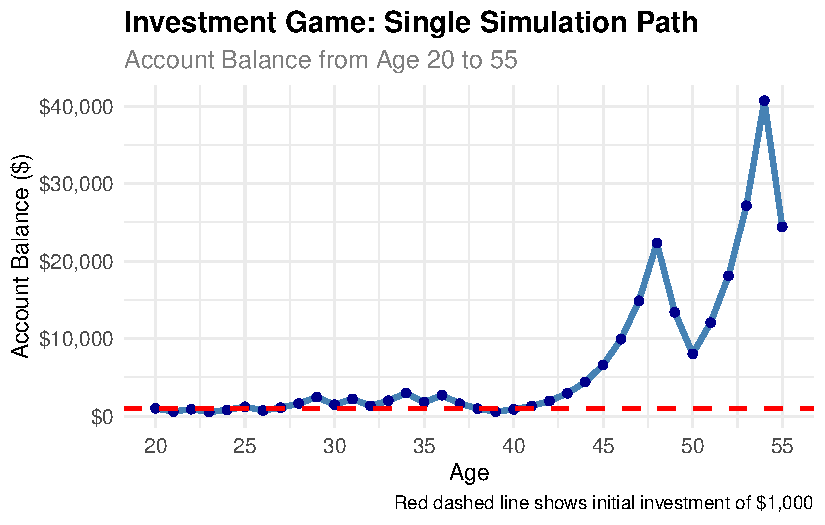
\includegraphics[keepaspectratio]{simulationmodel_files/figure-pdf/single-simulation-1.pdf}}

\begin{Shaded}
\begin{Highlighting}[]
\CommentTok{\# Show first few and last few years}
\FunctionTok{cat}\NormalTok{(}\StringTok{"}\SpecialCharTok{\textbackslash{}n}\StringTok{First 10 years:}\SpecialCharTok{\textbackslash{}n}\StringTok{"}\NormalTok{)}
\end{Highlighting}
\end{Shaded}

\begin{verbatim}

First 10 years:
\end{verbatim}

\begin{Shaded}
\begin{Highlighting}[]
\FunctionTok{print}\NormalTok{(simulation\_data[}\DecValTok{1}\SpecialCharTok{:}\DecValTok{11}\NormalTok{, }\FunctionTok{c}\NormalTok{(}\StringTok{"age"}\NormalTok{, }\StringTok{"balance"}\NormalTok{)])}
\end{Highlighting}
\end{Shaded}

\begin{verbatim}
   age  balance
1   20 1000.000
2   21  600.000
3   22  900.000
4   23  540.000
5   24  810.000
6   25 1215.000
7   26  729.000
8   27 1093.500
9   28 1640.250
10  29 2460.375
11  30 1476.225
\end{verbatim}

\begin{Shaded}
\begin{Highlighting}[]
\FunctionTok{cat}\NormalTok{(}\StringTok{"}\SpecialCharTok{\textbackslash{}n}\StringTok{Last 10 years:}\SpecialCharTok{\textbackslash{}n}\StringTok{"}\NormalTok{)}
\end{Highlighting}
\end{Shaded}

\begin{verbatim}

Last 10 years:
\end{verbatim}

\begin{Shaded}
\begin{Highlighting}[]
\FunctionTok{print}\NormalTok{(simulation\_data[(}\FunctionTok{nrow}\NormalTok{(simulation\_data)}\SpecialCharTok{{-}}\DecValTok{9}\NormalTok{)}\SpecialCharTok{:}\FunctionTok{nrow}\NormalTok{(simulation\_data), }\FunctionTok{c}\NormalTok{(}\StringTok{"age"}\NormalTok{, }\StringTok{"balance"}\NormalTok{)])}
\end{Highlighting}
\end{Shaded}

\begin{verbatim}
   age   balance
27  46  9929.163
28  47 14893.745
29  48 22340.618
30  49 13404.371
31  50  8042.622
32  51 12063.934
33  52 18095.900
34  53 27143.850
35  54 40715.776
36  55 24429.465
\end{verbatim}

\textbf{Comments on the Results:}

The results of the simulation were extremely positive! At age 55 I ended
with around \$25,000 in my account. However, my account experienced a
signficant drop during my last coin flip which resulted in my losing
\$15,000. While this last flip was painful, I'm still very happy overall
with the results!

\subsubsection{85\% Grade}\label{grade-1}

\begin{enumerate}
\def\labelenumi{\arabic{enumi}.}
\setcounter{enumi}{3}
\tightlist
\item
  \textbf{Multiple Simulations:} Run 100 simulations. Create a
  probability distribution plot of final balances at age 55.
\end{enumerate}

\begin{Shaded}
\begin{Highlighting}[]
\CommentTok{\# Your code here}
\end{Highlighting}
\end{Shaded}

\subsubsection{95\% Grade}\label{grade-2}

\begin{enumerate}
\def\labelenumi{\arabic{enumi}.}
\setcounter{enumi}{4}
\tightlist
\item
  \textbf{Probability Analysis:} What is the probability that your
  balance will be greater than \$1,000 at age 55?
\end{enumerate}

\begin{Shaded}
\begin{Highlighting}[]
\CommentTok{\# Your code here}
\end{Highlighting}
\end{Shaded}

\subsubsection{100\% Grade}\label{grade-3}

\begin{enumerate}
\def\labelenumi{\arabic{enumi}.}
\setcounter{enumi}{5}
\tightlist
\item
  \textbf{Strategy Comparison:} Run 100 simulations for the modified
  strategy. What is the probability of having more than \$10,000 at age
  55? Compare with the original game.
\end{enumerate}

\begin{Shaded}
\begin{Highlighting}[]
\CommentTok{\# Your code here}
\end{Highlighting}
\end{Shaded}





\end{document}
